\begin{pastexam}[label={px:ccu-110-csb-03}]{中正資工所乙組 110 學年度 第 3 題}
（問答）

(10\%) Given the following numbers: 75, 51, 80, 64, 10, 41, 92, 8, please answer the following
questions.
\begin{enumerate}[label=(\alph*)]
\item (7\%) Please sort these numbers in increasing order with the following \texttt{quicksort}
function, where the \texttt{swap} function is used to swap two numbers. Note that the first number
in each sublist is always selected as the pivot, and you must show necessary steps such that the
use of the \texttt{quicksort} function can be recognized.
\item (3\%) Assume that the numbers are input sequentially. Please construct a binary search tree
without rotations.
\end{enumerate}
\begin{minted}[fontsize=\small]{c}
void quicksort(int a[], int left, int right)
{
   int pivot, i, j;
   if (left < right) {
      i = left;
      j = right+1;
      pivot = a[left];
      do {
         do i++; while (a[i] < pivot);
         do j--; while (a[j] > pivot);
         if (i < j) swap(&a[i], &a[j]);
      } while (i < j);
      swap(&a[left], &a[j]);
      quicksort (a, left, j-1);
      quicksort (a, j+1, right);
   }
}
\end{minted}
\end{pastexam}

\begin{pastsoln}
\textbf{(a)} 排序結果 $8, 10, 41, 51, 64, 75, 80, 92$，過程見下面的表。

這個函式是 Horowitz 課本的寫法：基準取這一段的第一個數，$i$ 從左往右找「$\ge$ 基準」的數，$j$
從右往左找「$\le$ 基準」的數，$i < j$ 就交換，直到兩者交錯；最後把基準和 $a[j]$ 交換，基準就
落在最終位置 $j$。 和資結書虛擬碼~14.10 的 \proc{Hoare-Partition} 不同的地方是：最後多了一次
交換，把基準放到 $j$，遞迴時跳過 $j$。

\textbf{一個要先說明的細節}。 \texttt{do i++; while (a[i] < pivot);} 沒有檢查 $i \le
\mathit{right}$。 基準是這一段的最大值時，$i$ 會走出這一段，停在右邊第一個 $\ge$ 基準的數上。
這一段右邊如果還有數，它們都是之前的基準或它右邊的數，一定 $\ge$ 基準，$i$ 會停在那裡，不會出事；
但如果這一段就在陣列最右邊，$i$ 會讀到 \texttt{a[n]}，超出陣列。 Horowitz 課本的做法是事先在
\texttt{a[n]} 放一個比所有數都大的數當哨兵。 下面照這個假設追蹤（本題只有最後一次呼叫
\texttt{quicksort(a, 6, 7)} 用到）。 不管 $i$ 停在哪裡，只要 $i \ge j$ 迴圈就結束，答案不受影響。

陣列索引從 $0$ 開始，和 C 程式一致。 每一列是一次分割：$i$、$j$ 停下的位置寫成「$i\!=\!$ 位置
（值）」。

\begin{center}
\small
\begin{tabular}{lll}
\toprule
呼叫 & 步驟 & 陣列 $a[0..7]$ \\
\midrule
 & 開始 & 75, 51, 80, 64, 10, 41, 92, 8 \\
\addlinespace
$(0, 7)$ & 基準 $75$；$i\!=\!2$ (80)，$j\!=\!7$ (8)，交換 & 75, 51, \textbf{8}, 64, 10, 41, 92, \textbf{80} \\
基準 75 & $i\!=\!6$ (92)，$j\!=\!5$ (41)，$i > j$ 停 & \\
 & $a[0] \leftrightarrow a[5]$ & 41, 51, 8, 64, 10, \fbox{75}, 92, 80 \\
\addlinespace
$(0, 4)$ & 基準 $41$；$i\!=\!1$ (51)，$j\!=\!4$ (10)，交換 & 41, \textbf{10}, 8, 64, \textbf{51}, 75, 92, 80 \\
基準 41 & $i\!=\!3$ (64)，$j\!=\!2$ (8)，$i > j$ 停 & \\
 & $a[0] \leftrightarrow a[2]$ & 8, 10, \fbox{41}, 64, 51, 75, 92, 80 \\
\addlinespace
$(0, 1)$ & 基準 $8$；$i\!=\!1$ (10)，$j\!=\!0$ (8)，$i > j$ 停 & \\
基準 8 & $a[0] \leftrightarrow a[0]$（不變） & \fbox{8}, 10, 41, 64, 51, 75, 92, 80 \\
\addlinespace
$(3, 4)$ & 基準 $64$；$i\!=\!5$ (75)，$j\!=\!4$ (51)，$i > j$ 停 & \\
基準 64 & $a[3] \leftrightarrow a[4]$ & 8, 10, 41, 51, \fbox{64}, 75, 92, 80 \\
\addlinespace
$(6, 7)$ & 基準 $92$；$i\!=\!8$（哨兵），$j\!=\!7$ (80)，$i > j$ 停 & \\
基準 92 & $a[6] \leftrightarrow a[7]$ & 8, 10, 41, 51, 64, 75, 80, \fbox{92} \\
\bottomrule
\end{tabular}
\end{center}

框起來的數是這次分割的基準，放好之後不再移動。 表裡沒列的呼叫 $(0, -1)$、$(1, 1)$、$(3, 3)$、
$(5, 4)$、$(6, 6)$、$(8, 7)$ 都是 $\mathit{left} \ge \mathit{right}$，什麼都不做。 遞迴的
結構是
\[
(0,7) \to \bigl[(0,4) \to [(0,1),\ (3,4)],\ (6,7)\bigr],
\]
第一層以 $75$ 分成 $\langle 41, 51, 8, 64, 10\rangle$ 和 $\langle 92, 80\rangle$；左半再以 $41$
分成 $\langle 8, 10\rangle$ 和 $\langle 64, 51\rangle$。 注意 $(3, 4)$ 這段的 $i$ 走出了這一段，
停在第 $5$ 格的 $75$（上一層的基準），正是上面說的情形。

\textbf{(b)} 依序插入 $75, 51, 80, 64, 10, 41, 92, 8$，每個數從根往下比，小於往左、大於往右，
走到空的位置就放下（資結書虛擬碼~9.6）：
\begin{itemize}
\item $75$ 是根；$51 < 75$ 放左；$80 > 75$ 放右；
\item $64$：$< 75$ 往左，$> 51$ 放 $51$ 的右；$10$：$< 75$、$< 51$，放 $51$ 的左；
\item $41$：$< 75$、$< 51$、$> 10$，放 $10$ 的右；$92$：$> 75$、$> 80$，放 $80$ 的右；
\item $8$：$< 75$、$< 51$、$< 10$，放 $10$ 的左。
\end{itemize}
\begin{center}
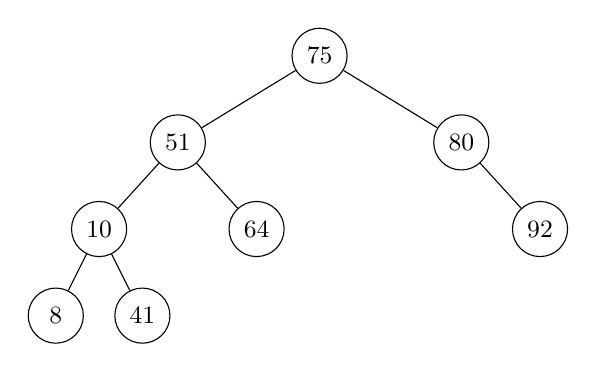
\begin{tikzpicture}[
  n/.style={circle,draw,minimum size=7mm,inner sep=0pt,font=\small},
  level distance=11mm,
  level 1/.style={sibling distance=36mm},
  level 2/.style={sibling distance=20mm},
  level 3/.style={sibling distance=11mm}]
\node[n] {75}
  child {node[n] {51}
    child {node[n] {10}
      child {node[n] {8}}
      child {node[n] {41}}}
    child {node[n] {64}}}
  child {node[n] {80}
    child[missing] {}
    child {node[n] {92}}};
\end{tikzpicture}
\end{center}
文字寫法是 $75\bigl(51(10(8, 41), 64),\; 80(-, 92)\bigr)$。 這棵樹的中序走訪
$8, 10, 41, 51, 64, 75, 80, 92$ 正好是 (a) 排好的結果。
\end{pastsoln}
